\documentclass{standalone}
\usepackage{stex}
\libinput{preamble}
\renewcommand{\labelitemi}{$\triangleright$}
\usepackage{stex-highlighting}
\usepackage{xcolor}
\newcommand{\blue}[1]{\textbf{\textcolor{blue}{#1}}}
\usepackage{tikz}
\begin{document}
\sf
\usemodule[courses/FAU/AI/course]{game-play/slides?evaluation-function}
\usemodule[smglom/search]{mod?heuristic}
\usemodule[courses/FAU/AI/course]{game-play/slides?minimax-algo}
\usemodule[courses/FAU/AI/course]{search/slides?id-search}
\usemodule[smglom/search]{mod?search-problem}
\usestructure{searchprob}
\usemodule[smglom/ai]{mod?decision-theory}
\begin{minipage}[t]{8.5cm}
  \blue{Note:} \sr{depth limit}{Depth-limited} \sn{minimax} requires an \sr{evaluation
    function}{evaluation} for every \sn{cut-off state} $s$.  If $s$ is terminal, we use
  its \sn{utility}, and otherwise an estimate.
\end{minipage}
\hskip 0.5cm
\scalebox{0.35}{
    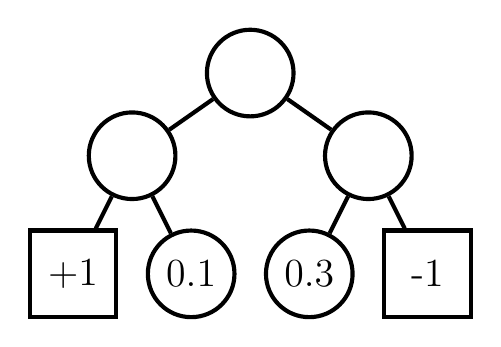
\begin{tikzpicture}[
        baseline={-4ex},
        scale=1.5, 
        every node/.style={draw, circle, inner sep=0pt, minimum size=1.1cm, line width=1.5pt},
    ]
        \node[shape=circle] (n0) at (0,-0.3) {};
        \node[shape=circle] (n1) at (-1,-1) {};
        \node[shape=circle] (n2) at (1,-1) {};
        \node[shape=rectangle] (n3) at (-1.5,-2) {\Large +1};
        \node[shape=circle] (n4) at (-0.5,-2) {\Large 0.1};
        \node[shape=circle] (n5) at (0.5,-2) {\Large 0.3};
        \node[shape=rectangle] (n6) at (1.5,-2) {\Large -1};
        \draw[line width=1.5pt] (n0) -- (n1);
        \draw[line width=1.5pt] (n0) -- (n2);
        \draw[line width=1.5pt] (n1) -- (n3);
        \draw[line width=1.5pt] (n1) -- (n4);
        \draw[line width=1.5pt] (n2) -- (n5);
        \draw[line width=1.5pt] (n2) -- (n6);
    \end{tikzpicture}
}
\end{document}
